% Utiliser des sections et des subsections pour les différentes parties du document.
% Utiliser begin{figure} pour les images sans oublier les labels pour le référencement

\section{Présentation générale}

\subsection{Archétype}

Notre but est de réaliser un jeu stratégique au tour par tour semblable à Advance Wars


\begin{figure}[h]
    \centering
    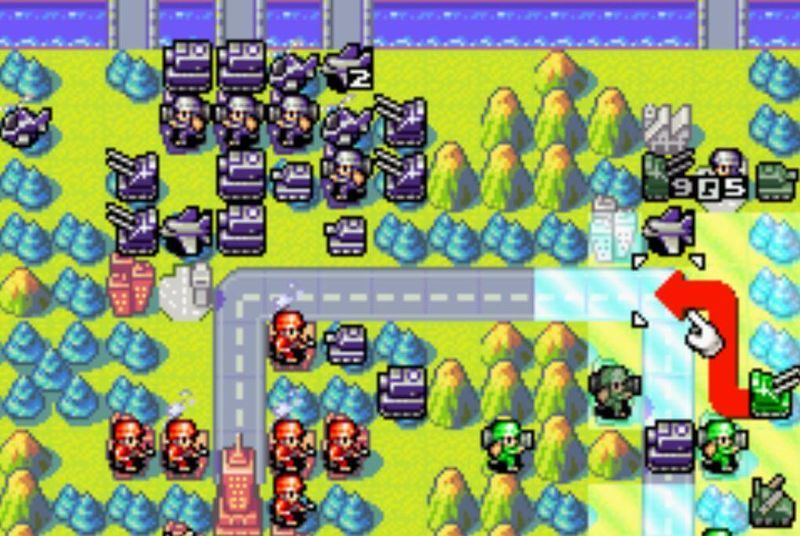
\includegraphics[scale = 0.5]{images/advanceWarsGameplay.jpg}
    \caption{Sprite des tuiles}
    \label{fig:Advance Wars}
\end{figure}


\subsection{Règles du jeu}

Notre jeu, "Until The Last Barrel", est un jeu de stratégie au tour par tour dont le but est de vaincre ses adversaires en capturant son Quartier Général (QG) sur le champ de bataille. Le dernier joueur survivant est donc déclaré vainqueur.
Pour se faire le joueur dispose de trois ressources: l'argent, le pétrole et des cartes.
\newpage

\subsubsection{Le champ de bataille}

Il s'agit d'une carte de tuiles (tile map) de différents types qui limitent ou améliorent la vitesse des unités des joueurs.
On peut notamment différencier les tuiles infranchissables comme les cours d'eau, et aussi les montagnes ou les forêts pour certaines unités, des plaines, chemins, routes et pont qui enjambent les cours d'eau.
Sur le champ de bataille se trouveront les QGs des joueurs, leurs unités, des villes, des usines et des puits de pétrole.



\paragraph{Les bâtiments}

Les bâtiments peuvent être capturés par les joueurs afin d'obtenir plus de ressources et autres avantages. Les puits de pétroles et les villes générent à chaque début de tour, respectivement du pétrol et de l'argent. Lorsqu'il veut jouer une carte le joueur peut placer des infanteries sur les villes et des unités motorisés sur les usines.



\subsubsection{Les ressources}

\paragraph{Les cartes}

Chaque joueur dispose d'un deck de carte duquel il pioche une carte à chaque début de tour. Une carte dispose d'un prix, qu'il est nécessaire de payer pour la jouer sur le champ de bataille, d'un type, de la description de ses effets. \n
\begin{itemize}
    \item \textbf{Les cartes unités} permettent pour un prix indiqué sur la carte d'invoquer sur le champ de bataille la dite unité. Dans le cadre des blindés, ceux-ci ne peuvent être invoqués qu'à proximité des usines.
    \item \textbf{Les cartes soutiens} se résolvent immédiatement sur n'importe quelle cible valide. Il peut s'agir d'un tir d'artillerie qui endommage des unités, à des soin ou encore de faire piocher le joueur.
    \item \textbf{Les cartes équipements} permettent d'améliorer les caractéristiques d'une unité alliée déjà présente sur le champ de bataille. 
    \item \textbf{Les cartes installations} sont un type de carte dont la fonction est de modifier les tuiles du champ de bataille. Il s'agit alors de pièges, bunker, pont, etc, afin de modifier le champ de bataille à son avantage. Les installations sont déployées à partir de certaines unités ayant la capacité nécessaire pour déployer l'installation voulue.

\end{itemize}


\paragraph{L'argent}

Au début de chaque tour, un joueur reçoit de l'argent en fonction de chaque ville qu'il a conquis, il peut alors dépenser cet argent lors de son tour afin de jouer des cartes. L'argent peut aussi être dépensé pour piocher des cartes.

\paragraph{Le pétrole}

Au début de chaque tour, un joueur reçoit du pétrole en fonction de chaque puit de pétrole qu'il possède, il peut alors utiliser ce pétrole pour déplacer des unités motorisées sur le champ de bataille. Si un joueur ne dispose pas de pétrole ces unités motorisées sont alors immobilisées voir détruites s'il s'agit d'unités aériennes.


\subsubsection{Les unités}
Il existe différentes unités jouables depuis sa main vers le champ de batailles avec différentes caractéristiques.\n 
De les unités de base ont : 
\begin{itemize}
    \item Des points de vie. L'unité est détruite si ses points de vie tombent à zéro.
    \item Des points de déplacement.
    \item Un niveau (conditionne les dégâts d'attaque par exemple).
    \item De la portée. Combien de tuiles peuvent être entre l'unité attaquante et l'unité attaquée.
    \item Des avantages face à certaines unités
    \item Des capacités spéciales
    \item Des équipements (ajoutés par d'autres cartes d'équipements)
\end{itemize}


\newpage
\subsection{Ressources}

Afin de pourvoir représenter les différentes unités, tuiles et autres éléments du jeu, nous avons crée par nous même des sprites. Nous utilisons une platte de 32 couleurs.

\begin{figure}[h]
    \centering
    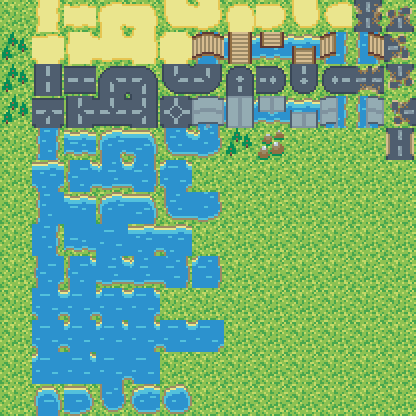
\includegraphics[scale = 1]{images/mapTileset.png}
    \caption{Sprite des tuiles}
    \label{fig:Advance Wars}
\end{figure}

\begin{figure}[h]
    \centering
    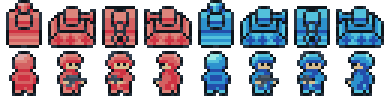
\includegraphics[scale = 1]{images/units.png}
    \caption{Sprite des unités}
    \label{fig:Advance Wars}
\end{figure}

\begin{figure}[h]
    \centering
    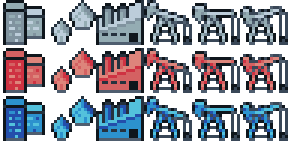
\includegraphics[scale = 1]{images/buildings.png}
    \caption{Sprite des bâtiments}
    \label{fig:Advance Wars}
\end{figure}

\clearpage

\section{Description et conception des états}

\subsection{Description des etats}

Un état du jeu est descrit par des éléments fixes (le champs de bataille), par un ensemble d'éléments mobiles (unités) et par les ressources des joueurs. Il existe aussi un compteur de tour afin de déterminer quel joueur peut jouer. On a donc:

\begin{itemize}
    \item Des coordonnées (x,y) pour les tuiles et les unités sur le champ de bataille
    \item Des classes différenciant les tuiles et les unités
    \item Des objets pour les joueurs déterminant les cartes, l'argent et le pétrole qu'ils possèdent.
    \item Un compteur pour les tours
\end{itemize}


\subsubsection{Eléments fixes}

Le champs de bataille est formé par une grille d'éléments nommé tuiles ou cases. La taille de la grille est fixée au démarrage de la partie. Les types de cases sont:

\begin{itemize}
    \item Les cases d'eau, de montagne et de forêt. Infranchissable par n'importe quelle unité.
    \item Les cases d'herbes qui permettent un déplacement standard.
    \item Les cases chemins qui permettent un déplacement plus rapide que celles d'herbe.
    \item Les cases routes qui permettent un déplacement plus rapide que celles d'herbe.
    \item Les ponts permettent de passer au dessus des cases d'eau et possèdent les mêmes caractéristiques que les chemins ou routes. Il existe.
    \item Les bâtiments se trouvent sur la carte. Ils peuvent soit être neutre, soit appartenir à un joueur. Parmis eux il existe: le QG, les usines, les villes et villages, et les puits de pétrole.
    \item Les installations sont des modifications du champs de bataille par les joueurs. Il peut s'agir de construire un pont, installer une barricade ou d'autres lignes de défence.
\end{itemize}

\newpage


\subsubsection{Eléments mobiles}
Les éléments mobiles autrement dit les unités possèdent une direction, un status fatigué, des points de mouvements, une position, des équipements, des PVs, un niveau, une spécialité. Les cartes sont elles aussi des éléments mobiles. En effet un joueur jouant une carte la fait passer de sa main au champs de bataille. \n
Il existe aussi des états intermédiaires quand le joueur décide de déplacer une unité ou jouer une carte.

\begin{itemize}
    \item Les points de mouvements autorise les déplacement selon le type de terrain. A zéro, l'unité est immobile.
    \item Le status "fatigué" (exhausted) pour savoir si l'unité peut entreprendre des actions ou non.
    \item Les PVs détermine si l'unité est en vie. A zéro l'unité est détruite et retirée du champs de bataille. 
    \item Le niveau est un état fixe qui détermine la puissance d'attaque de l'unité.
    \item Les équipements sont susceptibles de modifier les statistiques de l'unité équipé.
    
\end{itemize}


\subsubsection{Etat général}

Il existe quelques caractéristiques générales:

\begin{itemize}
    \item Un compteur de tour pour déterminer le joueur actif
    \item Un status "victoire" qui affiche au vainqueur et au vaincu la fin du jeu ainsi que son résultat.
    \item Une liste de joueurs ainsi qu'une liste des objets sur le champs de bataille.
\end{itemize}



\begin{figure}[h]
    \centering
    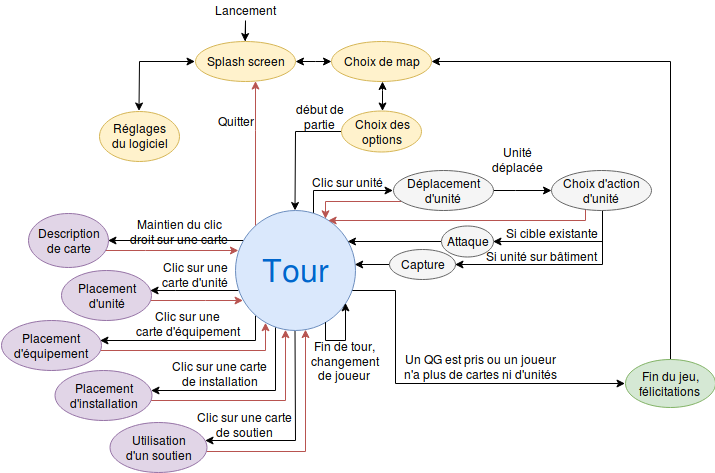
\includegraphics[scale =0.65]{images/etatsDeJeu.png}
    \caption{Diagramme du tour}
    \label{fig:Advance Wars}
\end{figure}



\newpage
\phantom{Texte invisible parce que j'ai pas trouvé d'autre méthode pour mettre le tableau à la ligne.}

\begin{tabularx}{15 cm}{|X|X|}
\hline
\textbf{GameState} \newline A pour but de décrire l'état du jeu & Attributs: map, players, existingCards, turn, allFieldObjects \newline Méthodes: GameState, getMap, EndTurn, Newturn, GenerateRessource, getPlayer\\ 
\hline
\textbf{FieldObjects} \newline C'est la liste qui contient tout les objets du champs de bataille & Attribut: fieldObjects(vecteur de FieldObject) \\
\hline
\textbf{FieldObject} \newline C'est la classe qui décrit tout les objets du champs de bataille: leur emplacement, l'image associée, le propriétaire et le type  & Attributs: position, sprite, owner, type \newline Méthodes: FieldObject, setOwner, getPosition, setObjectType\\
\hline
\textbf{Building} \newline Un bâtiment peut être capturé par des unités afin qu'un joueur en prenne le contrôle & Attribut: health \newline Méthode: Building, captured\\
\hline
\textbf{ObjectType} \newline C'est une classe dénumération des types possibles que peut prendre un FieldObject & Attributs: HEADQUARTER, TOWN, FACTORY, OILWELL, INSTALLATION, UNIT \newline \\
\hline
\textbf{Headquarter} & Attribut: moneyProduction \newline Méthodes: Headquarter, setMoneyProduction, captured, setMoneyProduction, getMoneyProduction\\
\hline
\textbf{Town} & Attribut: moneyProduction \newline Méthode:Town, Town (un deuxième constructeur), setMoneyProduction, setMoneyProduction, getMoneyProduction\\
\hline
\textbf{Factory} &  
\newline\\
\hline
\textbf{OilWell} & Attribut:oilProduction \newline Méthodes: OilWell, setOilProduction\\
\hline
\textbf{Installation} & Attribut: sourceCard \newline\\
\hline
\textbf{Unit} & Attributs: equipments, headcount, sourceCard \newline Méthodes:getHeadCount, move, attack, defence, capture\\

\hline
\textbf{Direction} \newline C'est une classe d'énumation qui permettra de changer les sprites en fonction des mouvements des unités & Attributs: UP, RIGHT, DOWN, LEFT \newline \\
\hline

\end{tabularx}



\begin{tabularx}{15 cm}{|X|X|}
\hline
\textbf{Map} & Attributs: tiles, size  \newline Méthodes: Map, Map (un deuxième constructeur)\\
\hline
\textbf{Tile} & Attributs: Speed  \newline Méthodes: Tile\\
\hline
\textbf{Tiles} & Attributs: tiles  \newline Méthodes: Tiles\\

\hline
\textbf{Player} & Attributs: deck, hand, money, oil, name, ownedFieldObjects, id, count  \newline Méthodes: Player, getMoney, setMoney, getOil, setOil, getId, addOwnedFieldObject, removeOwnedFieldObject\\
\hline
\textbf{Deck} & Attributs: cards  \newline Méthodes: Deck, Deck (deuxième constructeurs), pull, remove\\
\hline
\textbf{Cards} & Attributs: cards  \newline Méthodes: Cards, getCard\\
\hline
\textbf{Card} & Attributs: id, title, cost, decription, type  \newline Méthodes: Card, Card (un deuxième constructeur), playCard\\
\hline
\textbf{CardType} \newline Classe d'énumération pour différencier les types de cartes & Attributs: UNIT, EQUIPMENT, INSTALLATION, SUPPORT  \newline \\
\hline
\textbf{EquipmentCard} & Attributs: level, strengths, headCount  \newline Méthodes: EquipmentCard, playCard\\
\hline
\textbf{UnitCard} & Attributs:level, unitType, strengths, movesByTurn, oilCost  \newline Méthodes: UnitCard, playCard\\
\hline
\textbf{InstallationCard} & Attributs: stopOpponent, damage, iterations \newline Méthodes: InstallationCard, playCard\\
\hline
\textbf{SupportCard} & Attributs: damage, heal, moneyLoss, moneyGain, oilLoss, oilGain  \newline Méthodes: SupportCard, playCard\\
\hline
\end{tabularx}

\newpage

\begin{figure}[h]
    \centering
    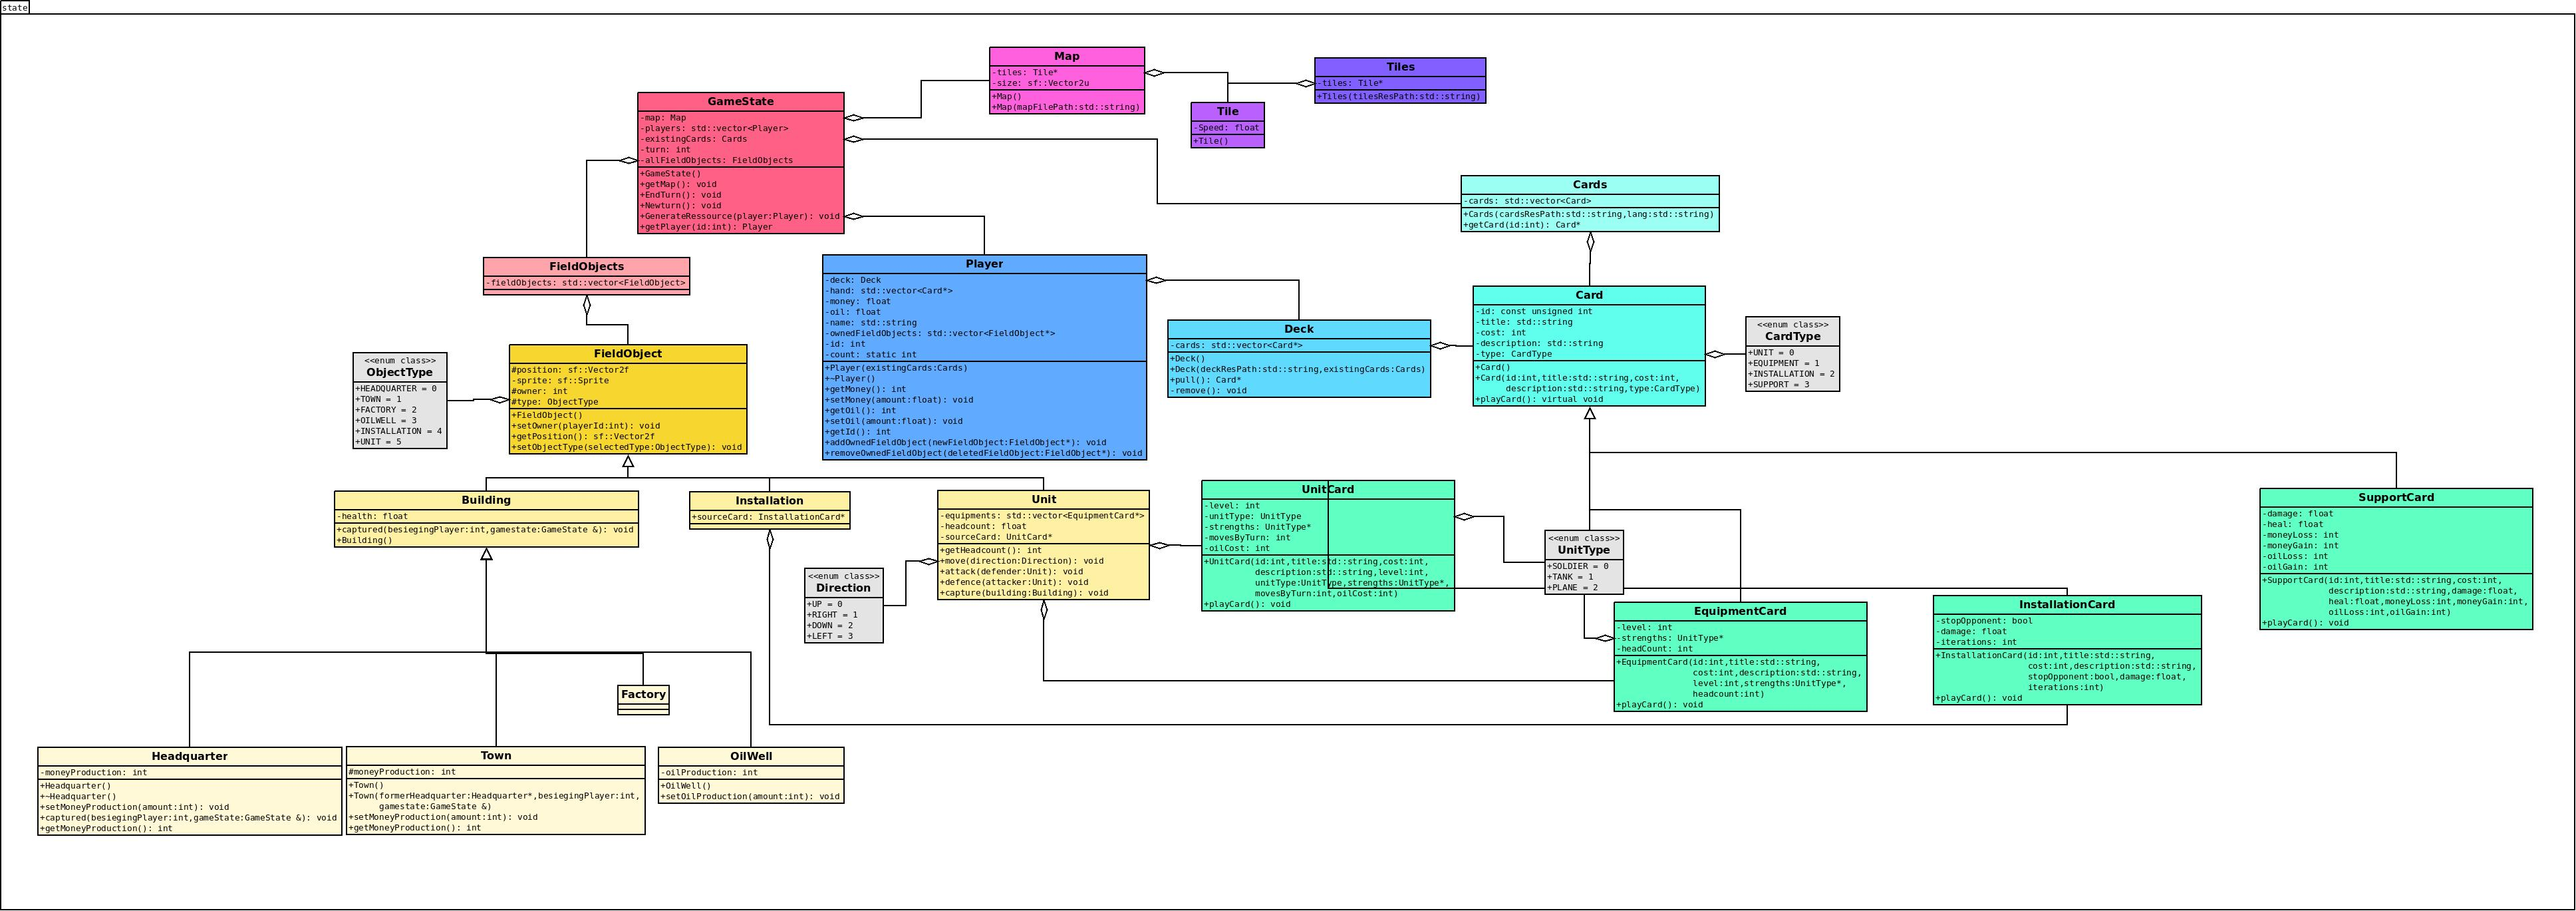
\includegraphics[angle=270,origin=c,scale =0.12]{images/state.jpeg}
    \caption{Diagramme UML de l'état}
    \label{fig:Advance Wars}
\end{figure}



\newpage







